% ============================================================
% Unidade 2 — Igualdade, inclusão e conjunto das partes   (didática v4 · kit/didatica.md §2)
% Parte A, o "artigo": Prefácio, De onde vem?, Onde é usado?
% IDs: 2-H1..H4 · 2-U1..U3 · 2-E1..E5 · 2-O1..O3 (matriz.yaml) · fonte única: dossies/u2.md
% ============================================================
\clearpage
\section{Igualdade, inclusão e conjunto das partes}

% ------------------------------------------------------------
\Prefacio
\begin{prefacio}
\gancho{Membro ou parte?}

O grêmio de uma escola tem uma comissão de cinco alunos, e dentro dela há uma subcomissão de dois alunos que cuida da festa junina. A subcomissão é \emph{membro} da comissão? Não: membros da comissão são os cinco alunos. A subcomissão é um grupo formado por alguns desses membros — é uma \emph{parte} da comissão. Quem confunde as duas coisas acaba contando seis membros onde há cinco.

Uma segunda pergunta, parecida. A lista de convidados \enquote{Ana, Bia, Caio} e a lista \enquote{Caio, Ana, Bia, Ana} convidam as mesmas pessoas? Sim: a ordem mudou e um nome apareceu duas vezes, mas quem está convidado é o mesmo.

As duas situações fazem a mesma pergunta em linguagem de conjuntos. \textbf{Quando dois conjuntos são o mesmo — e qual a diferença entre \emph{ser elemento} de um conjunto e \emph{ser parte} dele?} É o que esta unidade responde.

\textbf{Ao final, você será capaz de:} decidir se dois conjuntos são iguais; distinguir $\in$ de $\subset$, inclusive quando há chaves dentro de chaves; provar uma inclusão ou uma igualdade; listar e contar os subconjuntos de um conjunto.

\textbf{Pré-requisitos:} da Unidade~1, pertinência, descrição de conjuntos e conjunto vazio; do Capítulo I, o condicional (\enquote{se\ldots{} então}) e o bicondicional (\enquote{se e somente se}). O essencial está na caixa abaixo.
\end{prefacio}

\begin{minimo}
\begin{itemize}[leftmargin=1.4em,itemsep=1pt]
  \item \textbf{Pertinência e descrição.} $x\in A$ significa que $x$ é um dos elementos de $A$; $\{x\in U\mid P(x)\}$ é o conjunto dos elementos de $U$ que satisfazem $P$ (Unidade~1).
  \item \textbf{Condicional.} \enquote{se $p$, então $q$} só é falso quando $p$ é verdadeira e $q$ é falsa. Em particular, se $p$ é falsa, o condicional é verdadeiro, qualquer que seja $q$ (Cap.~I).
  \item \textbf{Bicondicional.} \enquote{$p$ se e somente se $q$} equivale a \enquote{se $p$, então $q$} \emph{e} \enquote{se $q$, então $p$} (Cap.~I).
\end{itemize}
\end{minimo}

% ------------------------------------------------------------
\DeOndeVem

\subsubsection{Por que alguém precisou disso}
Na Unidade~1, combinamos que um conjunto fica determinado por quais objetos pertencem a ele. Dessa ideia saem duas perguntas. A primeira: quando duas descrições diferentes dão o \emph{mesmo} conjunto? Sem uma resposta, a frase \enquote{o conjunto das soluções é\ldots} não teria sentido, porque o mesmo conjunto poderia ser escrito de muitos jeitos. A segunda: como falar de uma parte de um conjunto — os números pares dentro dos inteiros, os quadrados dentro dos retângulos — sem confundir essa parte com um elemento?

\subsubsection{Quando dois conjuntos são o mesmo}
Em 1908, quando apresentou a primeira lista de axiomas da teoria dos conjuntos, Ernst Zermelo pôs em primeiro lugar justamente a regra de igualdade: se todo elemento de um conjunto $M$ é elemento de um conjunto $N$, e vice-versa, então $M=N$. Na formulação dele, todo conjunto é determinado pelos seus elementos.\src{sepZermelo}\src{zermelo1908} Lida hoje, é o \textbf{axioma de extensionalidade}. Na prática escolar, é a regra que manda ignorar a ordem e as repetições numa lista.\src{fme}

\begin{construcao}[igualdade de conjuntos]{2-H1}
\begin{enumerate}[label=(\arabic*)]
  \item Se um conjunto é determinado por quem pertence a ele, dois conjuntos com exatamente os mesmos elementos são o mesmo conjunto: $A=B$ quando todo elemento de $A$ pertence a $B$ e todo elemento de $B$ pertence a $A$.\src{fme}
  \item Consequência: a ordem dos elementos não importa, $\{a,b,c,d\}=\{d,c,b,a\}$; e a repetição também não, $\{a,a,a,b,b\}=\{a,b\}$.\src{fme}
  \item Duas descrições diferentes podem dar o mesmo conjunto: $\{x\mid 2x+1=5\}=\{2\}$.\src{fme}
  \item Para mostrar que $A\neq B$, basta uma \textbf{testemunha}: um elemento que está em um dos conjuntos e não está no outro. Em $\{a,b,d\}\neq\{a,b,c,d\}$, a testemunha é $c$.\src{fme}
\end{enumerate}
\end{construcao}

\subsubsection{Ser elemento e ser parte}
Os símbolos que separam essas duas relações têm história. Em 1889, Giuseppe Peano usou um épsilon como sinal de pertinência e explicou que ele abreviava a palavra latina \emph{est}, \enquote{é}.\src{mactutorSym}\src{peano1889} Uma boa maneira de ler $a\in b$, até hoje, é \enquote{$a$ é \emph{um} dos $b$}: o 3 é um dos elementos de $\{1,3,5\}$. Na mesma época, o lógico Gottlob Frege, que já aparecia na Unidade~1, insistia numa distinção que, segundo ele, muitos lógicos e matemáticos não faziam: uma coisa é um objeto \emph{cair sob} um conceito (por exemplo, um certo animal ser um cavalo); outra é um conceito estar \emph{subordinado} a outro (por exemplo, todo cavalo ser um mamífero).\src{park2018} Lida hoje, é a diferença entre pertencer ($\in$) e estar contido ($\subset$).\src{park2018}

\begin{construcao}[subconjunto]{2-H2}
\begin{enumerate}[label=(\arabic*)]
  \item Um conjunto $A$ é \textbf{subconjunto} de $B$ quando \emph{todo} elemento de $A$ é também elemento de $B$:
\[
A\subset B\iff (\text{para todo }x,\ x\in A\Rightarrow x\in B).
\]
Lê-se \enquote{$A$ está contido em $B$} ou \enquote{$A$ é parte de $B$}; também se escreve $B\supset A$, \enquote{$B$ contém $A$}.\src{fme}
\begin{center}
\begin{tikzpicture}[scale=0.8]
\draw[acento,thick,fill=acentoclaro] (0,0) ellipse (2.0 and 1.15);
\draw[acento,thick,fill=white] (0.45,-0.05) ellipse (0.95 and 0.6);
\node at (1.95,1.0) {$B$};
\node at (0.45,-0.05) {$A$};
\node[right] at (2.6,0) {$A\subset B$};
\end{tikzpicture}
\end{center}
  \item A negação de $A\subset B$ é $A\not\subset B$ (\enquote{$A$ não está contido em $B$}): existe pelo menos um elemento de $A$ que não pertence a $B$. Assim como na igualdade, basta uma testemunha.\src{fme}
  \item Neste material, $A\subset B$ admite $A=B$: todo conjunto está contido em si mesmo ($A\subset A$).\src{fme}
  \item O vazio está contido em qualquer conjunto: a sentença \enquote{se $x\in\varnothing$, então $x\in A$} tem a hipótese sempre falsa e, por isso, é sempre verdadeira (condicional do Cap.~I). Logo $\varnothing\subset A$, para todo $A$.\src{fme}
  \item \textbf{$\in$ ou $\subset$?} O símbolo $\in$ liga um objeto a um conjunto; $\subset$ liga dois conjuntos. Em $\{a,b\}$, temos $a\in\{a,b\}$ e $\{a\}\subset\{a,b\}$, mas $\{a\}\notin\{a,b\}$, porque $\{a\}$ não é um dos elementos listados.
\end{enumerate}
Valem ainda três propriedades (para conjuntos quaisquer): $A\subset A$; se $A\subset B$ e $B\subset A$, então $A=B$; se $A\subset B$ e $B\subset C$, então $A\subset C$.\src{fme}
\end{construcao}

\begin{definicao}[subconjunto]
$A$ é \textbf{subconjunto} de $B$ ($A\subset B$) quando todo elemento de $A$ pertence a $B$. Se existe um elemento de $A$ que não pertence a $B$, escreve-se $A\not\subset B$.
\end{definicao}

\subsubsection{Como provar que dois conjuntos são iguais}
\begin{construcao}[igualdade por dupla inclusão]{2-H3}
\begin{enumerate}[label=(\arabic*)]
  \item Pela construção 2-H1, $A=B$ quer dizer \enquote{$x\in A$ se e somente se $x\in B$}. Pelo bicondicional do Cap.~I, isso é o mesmo que duas inclusões:\src{fme}
\[
A=B\iff (A\subset B\ \text{e}\ B\subset A).
\]
  \item Daí um método de prova. Para mostrar $A\subset B$, tome um elemento \emph{qualquer} de $A$ — sem escolher qual — e mostre que ele pertence a $B$. Para mostrar $A=B$, faça isso nos dois sentidos.
  \item Testar alguns elementos não prova uma inclusão: o \enquote{todo} da definição exige um argumento que sirva para qualquer elemento. Já para \emph{derrubar} uma inclusão, um único contraexemplo basta.
\end{enumerate}
\end{construcao}

\subsubsection{Todos os subconjuntos de uma vez}
\begin{construcao}[conjunto das partes]{2-H4}
\begin{enumerate}[label=(\arabic*)]
  \item O \textbf{conjunto das partes} de $A$, indicado por $\mathcal{P}(A)$, é o conjunto cujos elementos são todos os subconjuntos de $A$.\src{fme} O vazio e o próprio $A$ estão sempre entre eles.
  \item Para montar $\mathcal{P}(A)$, decida, para cada elemento de $A$, se ele \emph{entra} ou \emph{não entra} no subconjunto. Para $A=\{a,b\}$:
\begin{center}
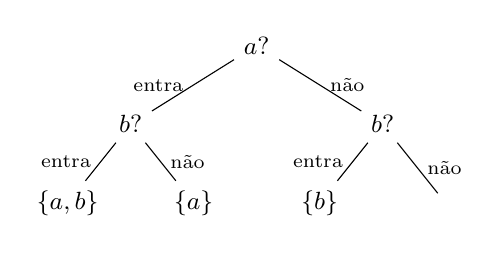
\begin{tikzpicture}[level distance=1.0cm, level 1/.style={sibling distance=3.2cm}, level 2/.style={sibling distance=1.6cm}, every node/.style={font=\small}]
\node {$a$?}
  child {node {$b$?} child {node {$\{a,b\}$} edge from parent node[left]{\scriptsize entra}} child {node {$\{a\}$} edge from parent node[right]{\scriptsize não}} edge from parent node[left]{\scriptsize entra}}
  child {node {$b$?} child {node {$\{b\}$} edge from parent node[left]{\scriptsize entra}} child {node {$\varnothing$} edge from parent node[right]{\scriptsize não}} edge from parent node[right]{\scriptsize não}};
\end{tikzpicture}
\end{center}
  \item Com $n$ elementos, são $n$ decisões de duas opções cada, e cada sequência de decisões dá um subconjunto diferente. Portanto,
\[
n\bigl(\mathcal{P}(A)\bigr)=\underbrace{2\cdot2\cdots2}_{n}=2^{n}.
\]
  \item Os elementos de $\mathcal{P}(A)$ são \emph{conjuntos}. Por isso, $X\in\mathcal{P}(A)$ significa exatamente $X\subset A$: é a ponte entre $\in$ e $\subset$.
\end{enumerate}
\end{construcao}

\begin{definicao}[conjunto das partes]
O \textbf{conjunto das partes} de $A$ é $\mathcal{P}(A)=\{X\mid X\subset A\}$. Se $A$ tem $n$ elementos, $\mathcal{P}(A)$ tem $2^n$ elementos.
\end{definicao}

\begin{paralembrar}\label{lembrar-u2}
\textbf{Dois conjuntos são iguais quando têm os mesmos elementos; ser parte ($\subset$) é \enquote{todo elemento de um está no outro}; ser elemento ($\in$) é \enquote{ser um dos listados}.}
\begin{enumerate}[label=\arabic*.,leftmargin=1.4em,itemsep=1pt]
  \item Para provar $A=B$, prove $A\subset B$ e $B\subset A$.
  \item Para provar $A\subset B$, tome um elemento qualquer de $A$ e mostre que ele está em $B$; para provar $A\not\subset B$, basta uma testemunha.
  \item Para contar subconjuntos, decida elemento a elemento: $2^n$.
\end{enumerate}
\end{paralembrar}

% ------------------------------------------------------------
\OndeEUsado

As ideias desta unidade aparecem em três tipos de enunciado: os que pedem para classificar sentenças com $\in$ e $\subset$, os que pedem uma justificativa ou uma prova, e os que pedem para contar subconjuntos.

\subsubsection{Mapa do problema}

\begin{caso}{1 · \enquote{classifique em V ou F} com $\in$ e $\subset$}{2-U1}
\mapa{sentenças com $\in$, $\notin$, $\subset$, $\not\subset$, muitas vezes com chaves dentro de chaves}
{o que está do lado esquerdo do símbolo: um objeto (pergunta de $\in$) ou um conjunto (pergunta de $\subset$)}
{2-H2 (5): $\in$ procura na lista de elementos; $\subset$ testa cada elemento}
\reconhecer O comando costuma ser seco: \enquote{Diga se é verdadeira (V) ou falsa (F) cada uma das sentenças abaixo}.\src{fme} O sinal é a mistura de símbolos e de chaves: $\{a\}$ pode ser elemento de um conjunto (se estiver listado) e também subconjunto (se $a$ estiver listado). Leia cada sentença em voz alta — \enquote{é um dos elementos?} ou \enquote{todos os elementos estão lá?} — antes de responder. Treino: \exref{ex:u2:chaves}; questões \ref{u2:fme20} e \ref{u2:fme47}.
\end{caso}

\begin{caso}{2 · \enquote{prove}, \enquote{mostre}, \enquote{justifique}}{2-U2}
\mapa{\enquote{mostre que $A\subset B$}, \enquote{prove que $A=B$}, \enquote{classifique e justifique}}
{o \enquote{todo} escondido na definição de $\subset$ e um elemento genérico}
{2-H3: elemento qualquer, ida e volta; testemunha para $\not\subset$}
\reconhecer O verbo pede um argumento, não uma conta. Se a sentença é de inclusão e você acha que é verdadeira, a justificativa precisa valer para \emph{todo} elemento; se acha que é falsa, uma testemunha basta. Treino: \exref{ex:u2:fme18} e \exref{ex:u2:multiplos}; \qref{u2:multiplos4}.
\end{caso}

\begin{caso}{3 · \enquote{quantos subconjuntos\ldots?}}{2-U3}
\mapa{\enquote{quantos subconjuntos}, \enquote{quantos conjuntos $X$ satisfazem $A\subset X\subset B$}, \enquote{de quantas maneiras escolher alguns de\ldots}}
{quais elementos são obrigatórios, quais são proibidos e quais são livres}
{2-H4: cada elemento livre dobra a contagem; com $k$ livres, $2^k$}
\reconhecer O sinal é uma escolha de \enquote{alguns} elementos sem ordem, com ou sem restrições. Em vez de listar, separe os elementos em três grupos — os que precisam entrar, os que não podem entrar e os livres — e conte só as decisões livres. Treino: \exref{ex:u2:partes}; questões \ref{u2:fme35} e \ref{u2:contar}.
\end{caso}

\subsubsection{Tabela de gatilhos}
\begin{gatilhos}
\enquote{V ou F} com chaves aninhadas & 2-H2 (5) & $\in$ procura na lista; $\subset$ testa cada elemento & \mbox{2-U1\,·\,q.\,\ref{u2:fme20}}\\\fino
\enquote{prove}, \enquote{mostre}, \enquote{justifique} & 2-H3 & elemento genérico, ida e volta & \mbox{2-U2\,·\,q.\,\ref{u2:multiplos4}}\\\fino
\enquote{não está contido} & 2-H2 (2) & procurar uma testemunha & \mbox{2-E3\,·\,q.\,\ref{u2:exemplos}}\\\fino
\enquote{quantos subconjuntos} & 2-H4 & contar os elementos livres: $2^k$ & \mbox{2-U3\,·\,q.\,\ref{u2:fme35}}\\
\end{gatilhos}
